%! TeX root = /Users/trustinnguyen/Downloads/Berkeley/Math/Math128a/Homework/Math128aHw8/Math128aHw8.tex

\documentclass{article}
\usepackage{/Users/trustinnguyen/.mystyle/math/packages/mypackages}
\usepackage{/Users/trustinnguyen/.mystyle/math/commands/mycommands}
\usepackage{/Users/trustinnguyen/.mystyle/math/environments/article}
\graphicspath{{./figures/}}

\title{Math128aHw8}
\author{Trustin Nguyen}

\begin{document}

    \maketitle

\reversemarginpar

\section*{Exercise Set 4.6}
\hrule

\textbf{Exercise 6}: Use Adaptive quadrature to approximate the following integrals to within $10^{-5}$.
    \begin{itemize}
        \item [(d)] $\int_{0}^{\pi/2} (6\cos{4x} + 4 \sin{6x})e^{x} \, \dd{x}$
    \end{itemize}
    I got: $5.1138387475811616517766680276784$. Here is the code:
    \inputminted{matlab}{./code/AdaptiveQuadrature/Simpson.m}
    \inputminted{matlab}{./code/script1.m}

\textbf{Exercise 9}: Sketch the graphs of $\sin{1 / x}$ and $\cos{1 / x}$ on $[0, 1, 2]$. Use Adaptive quadrature to approximate the following integrals to within $10^{-3}$.
    \begin{answer}
        For $\sin{1 / x}$, I got $1.3847974535053240059417414299214$ and for $\cos{1 / x}$, I got $0$.
        \begin{center}
            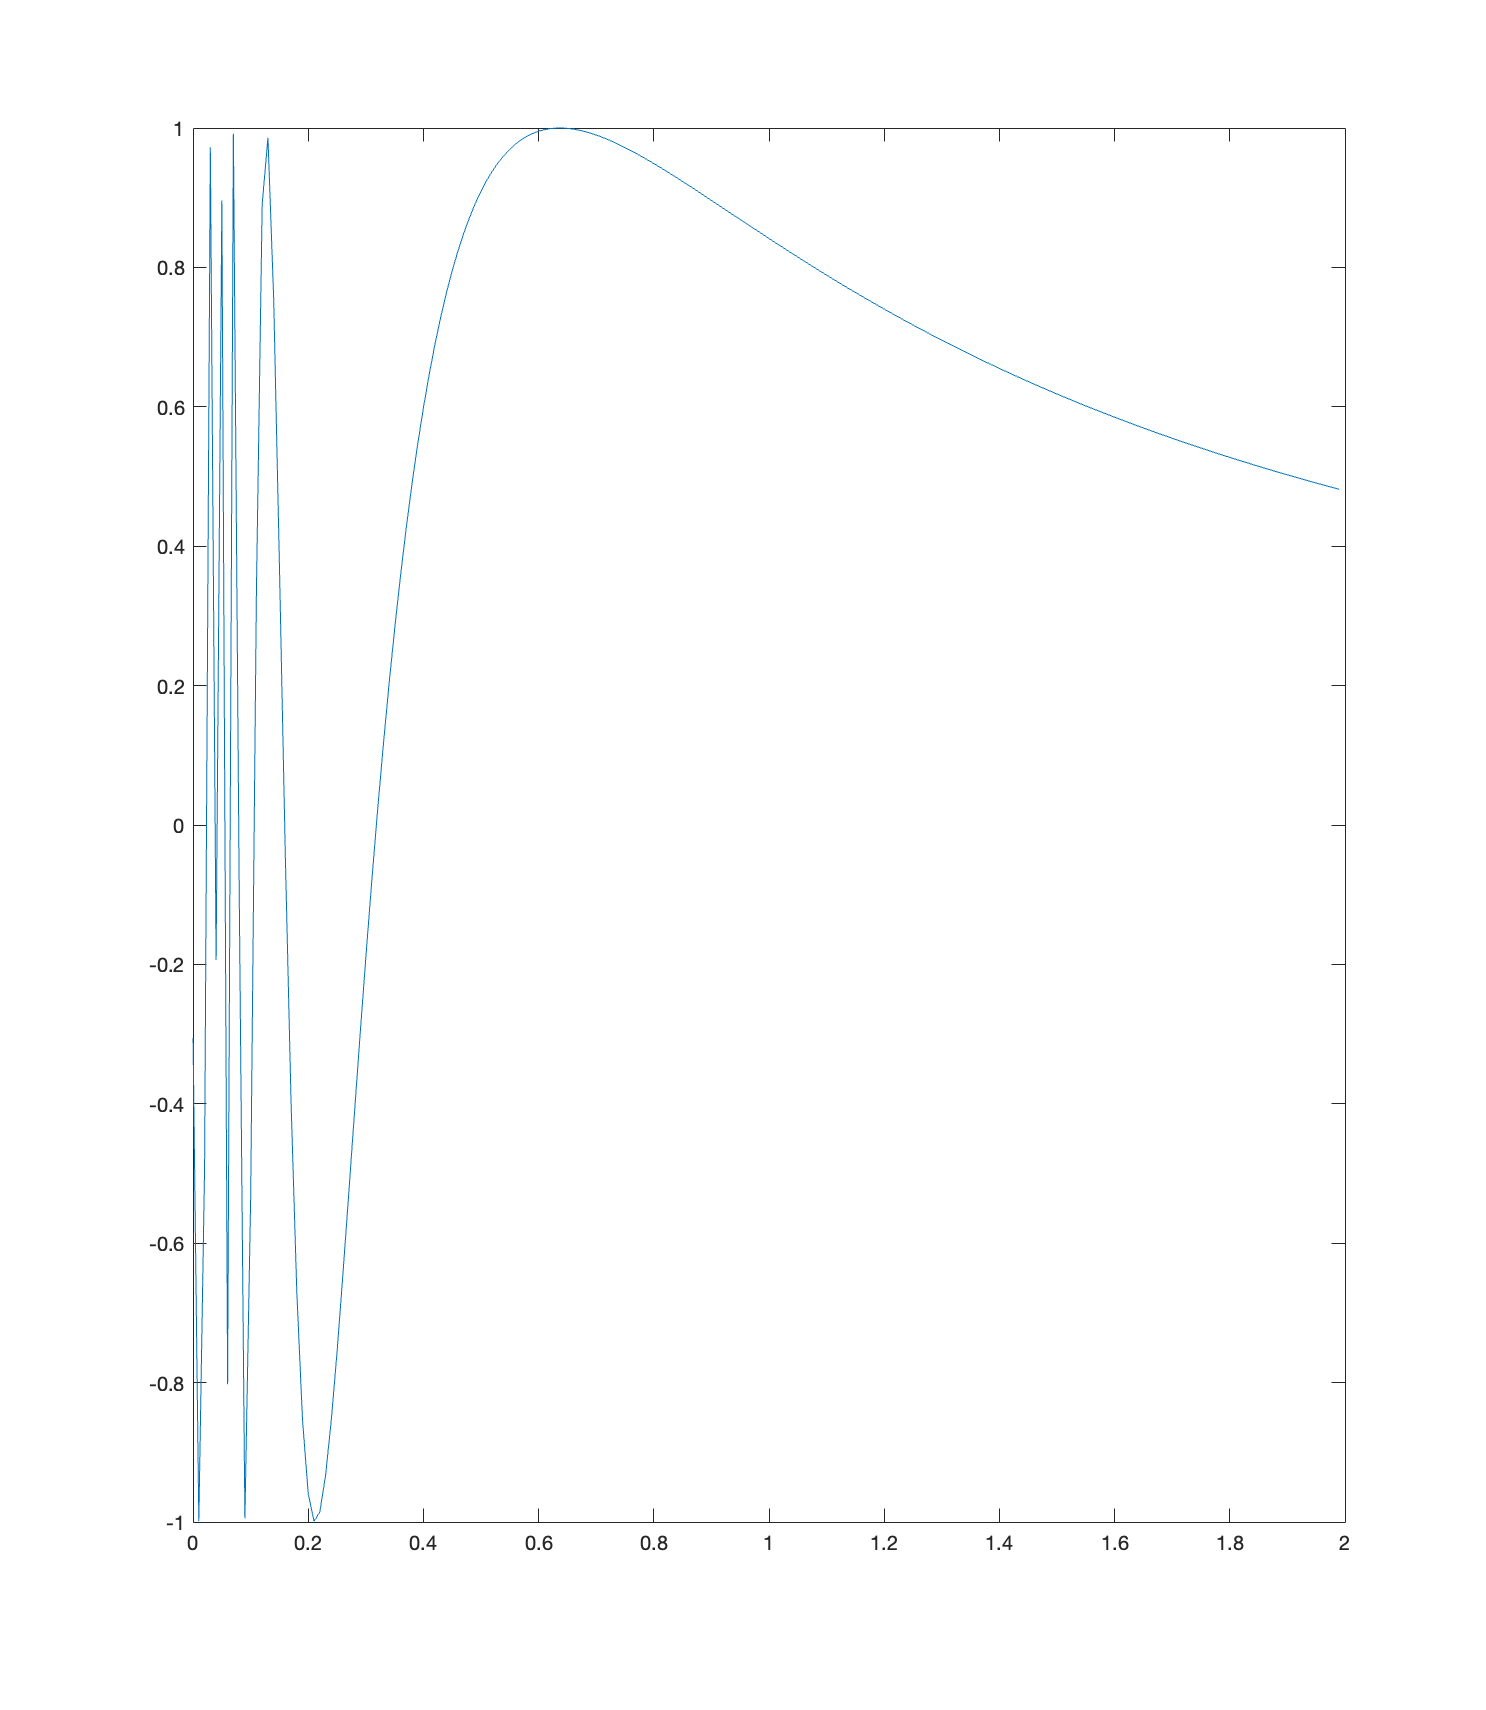
\includegraphics[scale=0.1]{sin1overx}
            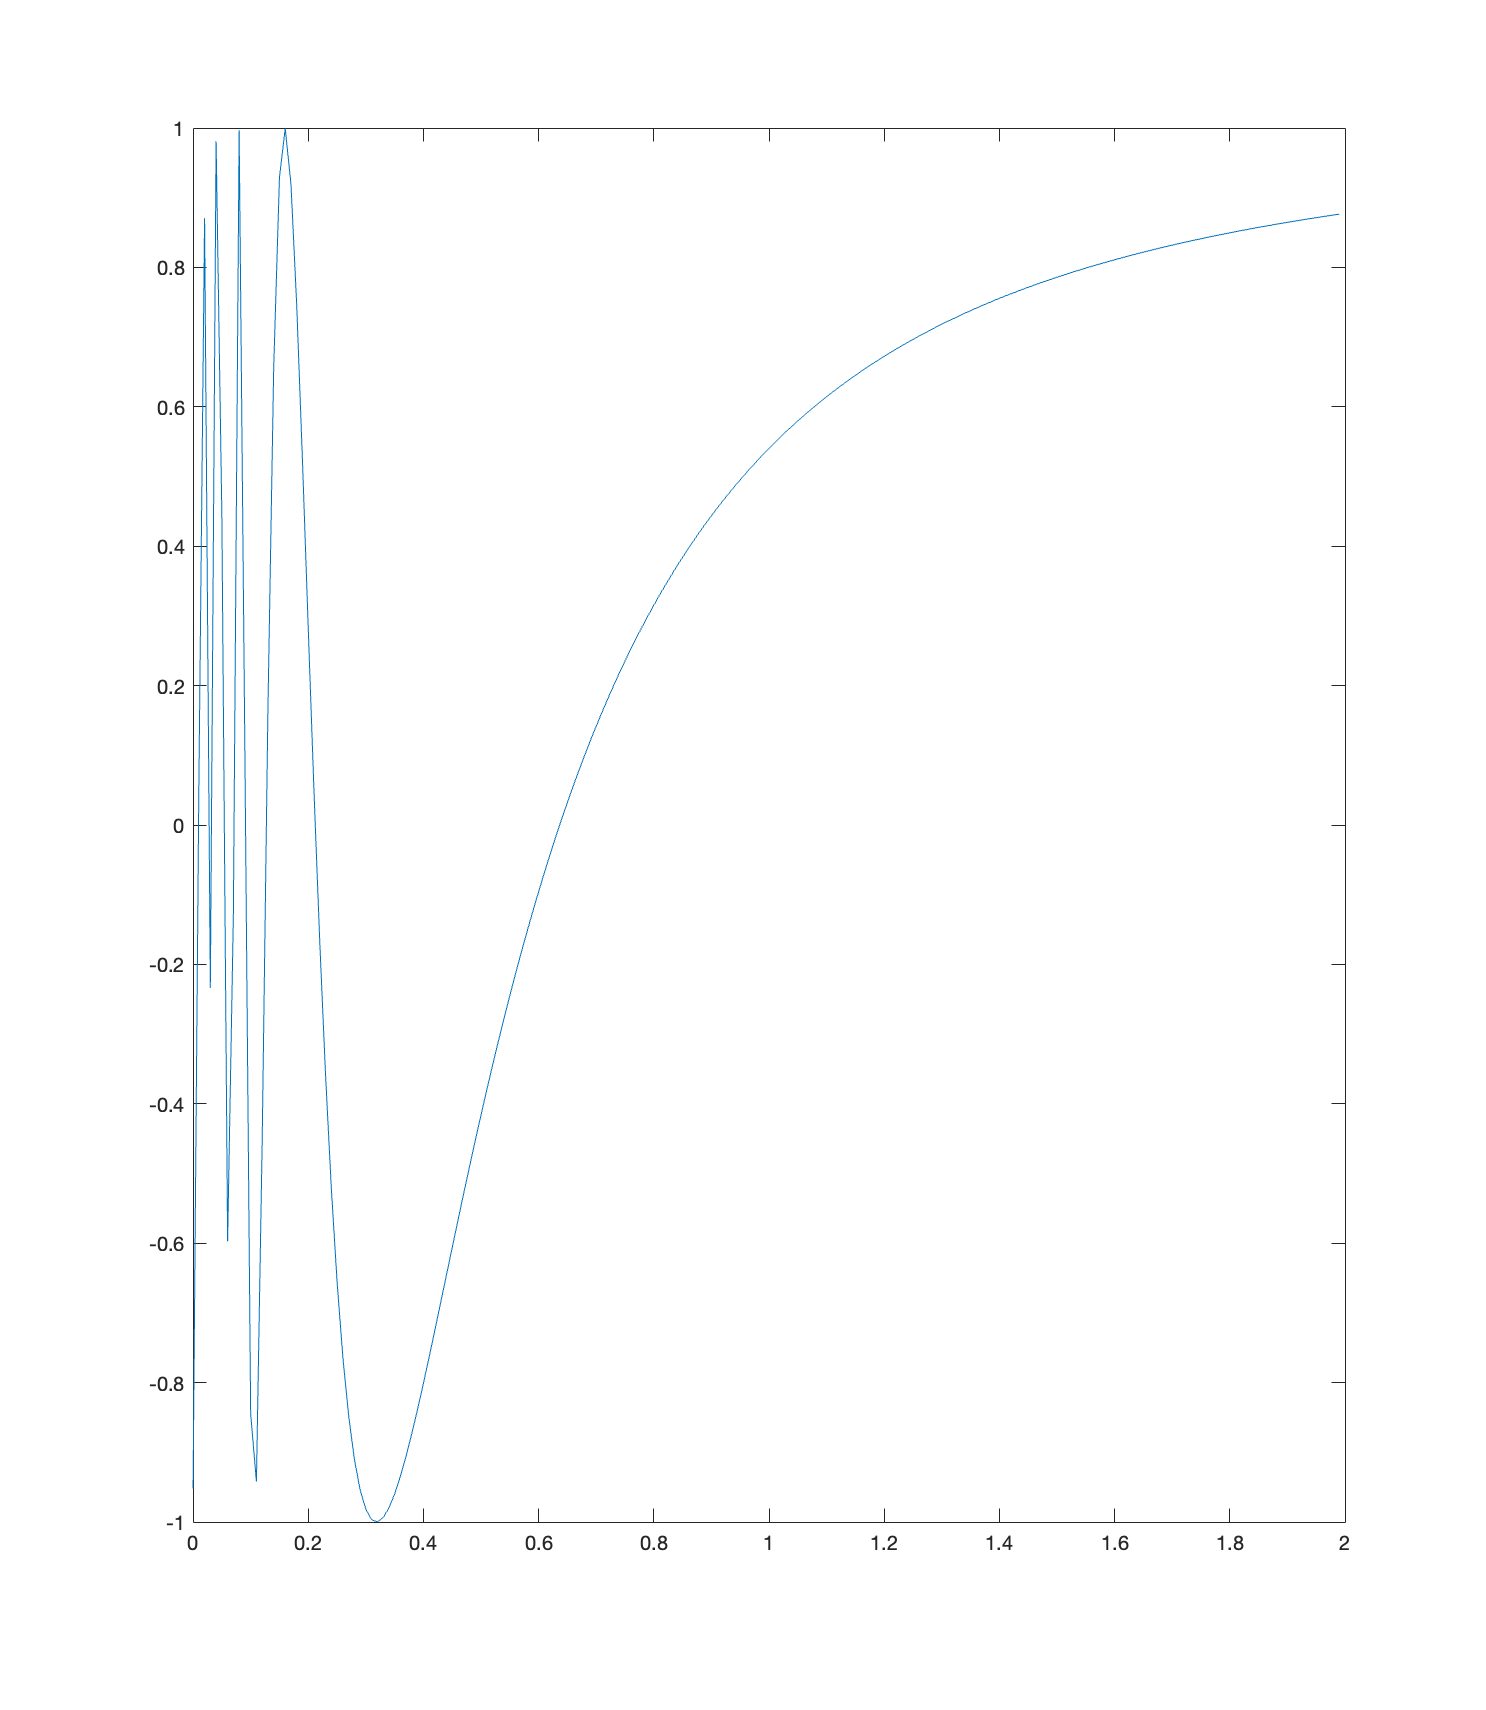
\includegraphics[scale=0.1]{cos1overx}
        \end{center}
    \end{answer}

\textbf{Exercise 11}: The differential equation 
    \begin{equation*}
        mu^{\prime\prime}(t) + ku(t) = F_{0} \cos{\omega t}
    \end{equation*}
describes a spring-mass system with mass $m$, spring constant $k$, and no applied damping. The term $F_{0} \cos{\omega t}$ describes a periodic external force applied to the system. The solution to the equation when the system is initially at rest $(u^{\prime}(0) = u(0) = 0)$ is
    \begin{equation*}
        u(t) = \dfrac{F_{0}}{m(\omega_{0}^{2} - \omega^{2})}(\cos{\omega t - \cos{\omega_{0}t}}), \, \text{where } \omega_{0} = \sqrt{\dfrac{k}{m}} \neq \omega
    \end{equation*}
Sketch the graph of $u$ when $m = 1, k = 9, F_{0} = 1, \omega = 2$, and $t \in [0, 2\pi]$. Approximate $\int_{0}^{2\pi} u(t) \, \dd{t}$ to within $10^{-4}$.
    \begin{answer}
        Integrating yields: $0.00017441076341495540713583292051187$.
        \begin{center}
            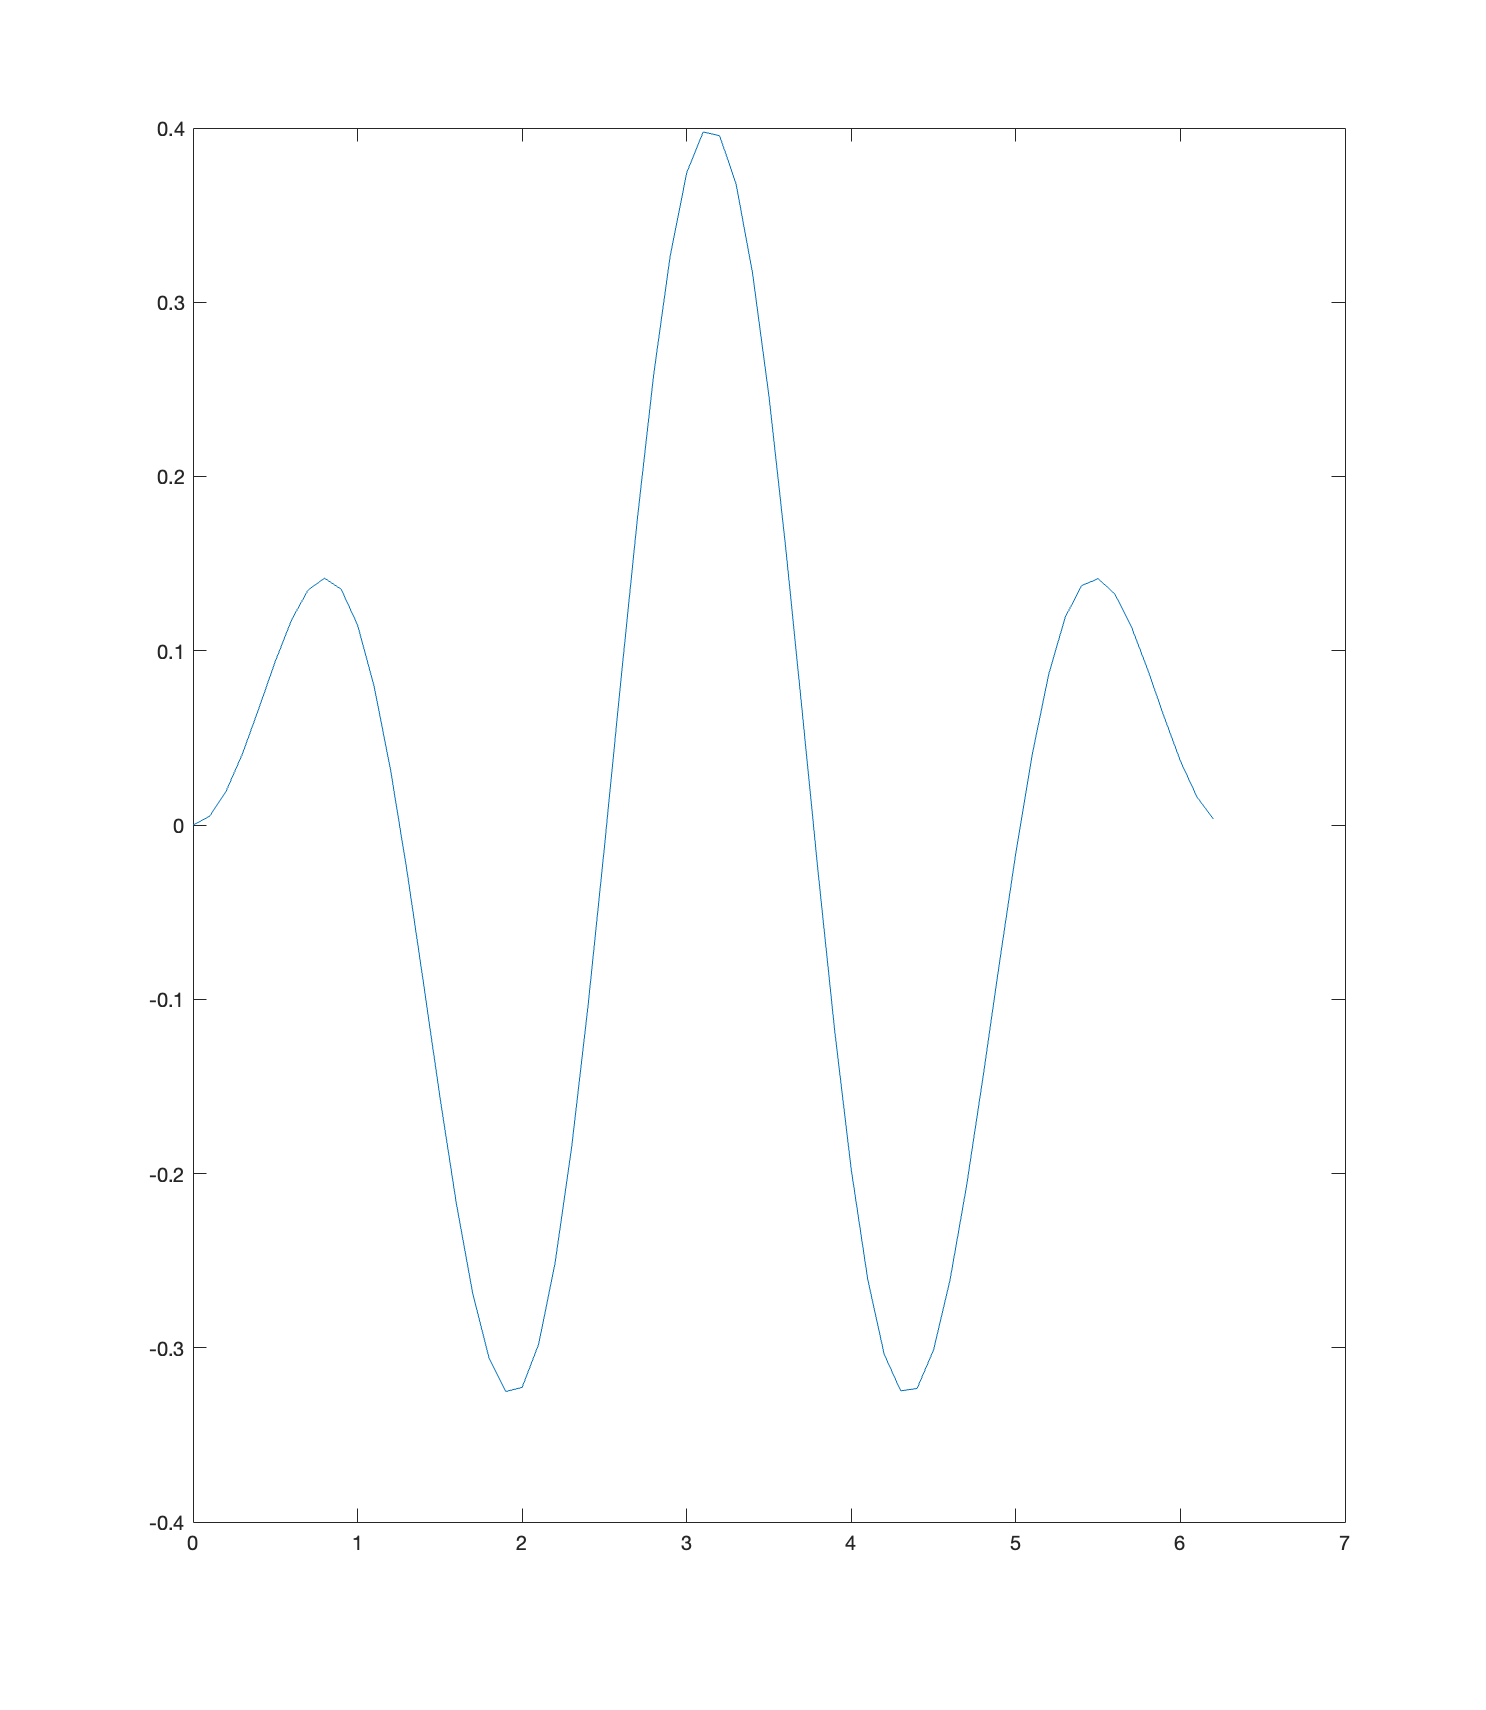
\includegraphics[scale=0.2]{spring_mass}
        \end{center}
    \end{answer}

\textbf{Exercise 13}: Let $T(a, b)$ and $T(a, \frac{a + b}{2}) + T(\frac{a + b}{2})$ be the single and double applications of the Trapezoidal rule to $\int_{a}^{b} f(x) \, \dd{x}$. Derive the relationship between
    \begin{equation*}
        \left\lvert T(a, b) - T\left(a, \dfrac{a + b}{2}\right) - T\left(\dfrac{a + b}{2}, b\right) \right\rvert
    \end{equation*}
and
    \begin{equation*}
        \left\lvert \int_{a}^{b} f(x) \, \dd{x} - T\left(a, \dfrac{a + b}{2}\right) - T\left(\dfrac{a + b}{2}, b\right) \right\rvert
    \end{equation*}
    \begin{answer}
        Using the error formula:
            \begin{equation*}
                \int_{a}^{b} f(x) \, \dd{x} = \dfrac{h}{2}[f(x_{0}) + f(x_{1})] - \dfrac{h^{3}}{12}f^{\prime\prime}(\mathcal{E}) = T(a, b) - \dfrac{h^{3}}{12}f^{\prime\prime}(\mathcal{E})
            \end{equation*}
        It can be seen that they differ by
            \begin{equation*}
                \left\lvert \dfrac{h^{3}}{12}f^{\prime\prime}(\mathcal{E}) \right\rvert
            \end{equation*}
    \end{answer}

\newpage
\section*{Exercise Set 4.7}
\hrule

\textbf{Exercise 2}: Approximate the following integrals using Gaussian quadrature with $n = 2$ and compare your results to the exact values of the integrals.
    \begin{itemize}
        \item [(c)] $\int_{0}^{3.5} \frac{x}{\sqrt{x^{2} - 4}} \, \dd{x}$
    \end{itemize}
    \begin{answer}
        I got: $-0.17681898945491190314095684640636$. Here is my code:
        \inputminted{matlab}{./code/gaussianQuadrature/gaussianQuad.m}
        \inputminted{matlab}{./code/script6.m}
    \end{answer}

\textbf{Exercise 6}: Repeat Exercise $2$ with $n = 4$.
    \begin{itemize}
            \item [(c)] $\int_{0}^{3.5} \frac{x}{\sqrt{x^{2} - 4}} \, \dd{x}$
    \end{itemize}
    \begin{answer}
        I got $-0.1768200201168954788441443888858$.
    \end{answer}

\textbf{Exercise 11}: Determine constants $a, b, c$, and $d$ that will produce a quadrature formula
    \begin{equation*}
        \int_{-1}^{1} f(x) \, \dd{x} = af(-1) + bf(1) + cf^{\prime}(-1) + df^{\prime}(1)
    \end{equation*}
that has degree of precision three.
    \begin{answer}
        Evaluate the integral for $f(x) = 1, x, 3x^{2}, x^{3}$:
            \begin{align*}
                \int_{-1}^{1} 1 \, \dd{x}      &= 2                        \\
                \int_{-1}^{1} x \, \dd{x}      &= 0                        \\
                \int_{-1}^{1} 3x^{2} \, \dd{x} &= x^{3} \eval_{-1}^{1} = 2 \\
                \int_{-1}^{1} x^{3} \, \dd{x}  &= 0                          
            \end{align*}
        Now evaluate the expression 
            \begin{equation*}
                af(-1) + bf(1) + cf^{\prime}(-1) + df^{\prime}(1)
            \end{equation*}
        for $f(x) = 1, x, 3x^{2}, x^{3}$:
            \begin{align*}
                f(-1)          &= 1, -1, 3, -1 \\
                f(1)           &= 1, 1, 3, 1   \\
                f^{\prime}(-1) &= 0, 1, -6, 3  \\
                f^{\prime}(1)  &= 0, 1, 6, 3     
            \end{align*}
        So we have the linear system:
            \begin{equation*}
                \begin{bmatrix}
                    1  & 1 & 0  & 0 \\
                    -1 & 1 & 1  & 1 \\
                    3  & 3 & -6 & 6 \\
                    -1 & 1 & 3  & 3   
                \end{bmatrix}\begin{bmatrix}
                    a \\
                    b \\
                    c \\
                    d   
                \end{bmatrix} = \begin{bmatrix}
                    2 \\
                    0 \\
                    2 \\
                    0   
                \end{bmatrix}
            \end{equation*}
        Solving this gives:
            \begin{equation*}
                \begin{bmatrix}
                    a \\
                    b \\
                    c \\
                    d   
                \end{bmatrix} = \begin{bmatrix}
                    1     \\
                    1     \\
                    1 / 3 \\
                    -1/ 3   
                \end{bmatrix}
            \end{equation*}
    \end{answer}


\textbf{Exercise 14}: Show that the formula $Q(P) = \sum_{i = 1}^{n} c_{i}P(x_{i})$ cannot have degree of precision greater than $2n - 1$ regardless of the choice of $c_{1}, \ldots, c_{n}$ and $x_{1}, \ldots, x_{n}$.

\newpage
\section*{Exercise Set 4.8}
\hrule

Section 4.8: Problems 1bc, 2bc, 17



\end{document}
